% Chapter Template

\chapter{MODI} % Main chapter title

\label{Chapter3} % Change X to a consecutive number; for referencing this chapter elsewhere, use \ref{ChapterX}

\lhead{Capítulo 3. \emph{MODI}} % Change X to a consecutive number; this is for the header on each page - perhaps a shortened title

%----------------------------------------------------------------------------------------
%	SECTION 1
%----------------------------------------------------------------------------------------

\section{Setup}

Se desea hacer realizar una investigación sobre el comportamiento colectivo de un grupo de robots, en el mundo real sin hacer uso de simuladores. Por esto  es necesario contar con un lugar físico donde poder activar los robot. Además para simplificar cada uno de los robots, estos no tienen sensores internos por lo que hay una cámara montada sobre el plano de movimiento de los robots, para hacer Seguimiento Visual.
\begin{figure}[htbp]
	\centering
		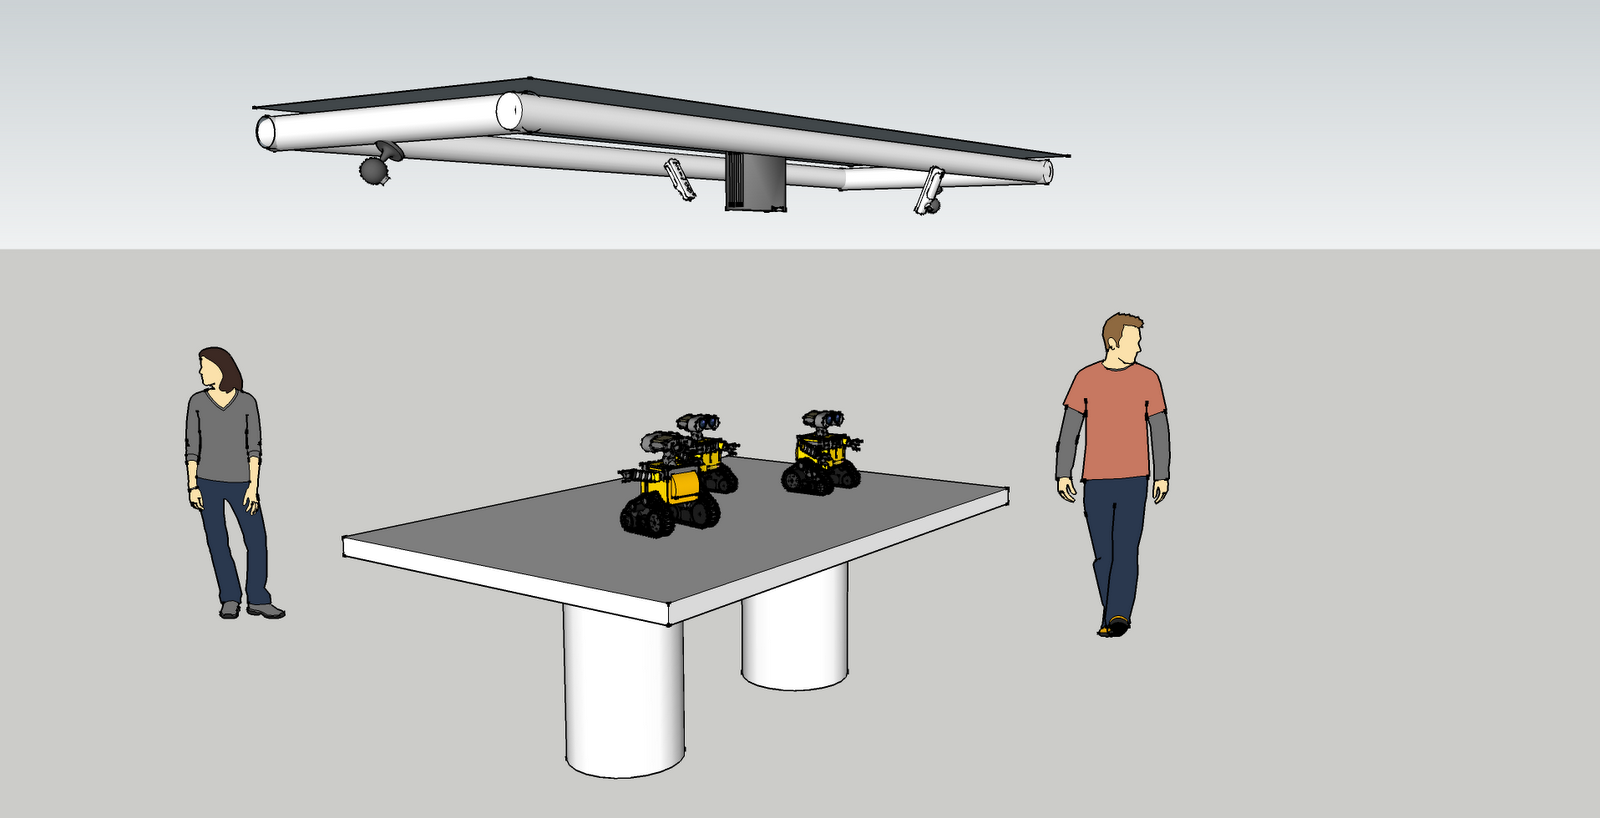
\includegraphics[width=0.8\textwidth]{./Figures/setup.png}
		\rule{35em}{0.5pt}
	\caption[Setup]{Setup a montarse para hacer estudios de grupos de robots.}
	\label{fig:setup}
\end{figure}

La función principal de MODI es ser una plataforma móvil de fácil acceso. Existe un repositorio en GitHub donde se tienen los códigos actualizados para controlar y construir robots MODI.  

\textbf{Las funciones principales que se desarrollaron}

\begin{itemize}
\item Carga Autónoma con celda solar.
\item Seguimiento de grupo.
\item Control individual del color de cada MODI.
\item Movimiento simple de cada robot de forma independiente.
\end{itemize}

%-----------------------------------
%	SECTION 2
%-----------------------------------

\section{Construcción}

%-----------------------------------
%	SUBSECTION 2
%-----------------------------------
\subsection{Fabricación Digital vs Análoga}

\begin{figure}[htbp]
	\centering
		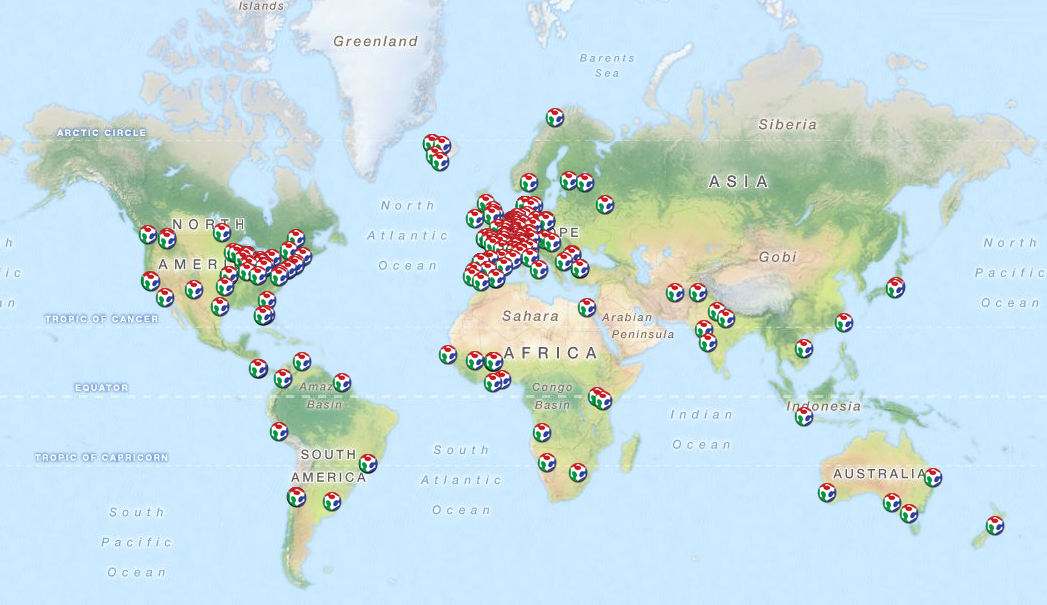
\includegraphics[width=0.8\textwidth]{./Figures/map.png}
		\rule{35em}{0.5pt}
	\caption[Setup]{Setup a montarse para hacer estudios de grupos de robots.}
	\label{fig:setup}
\end{figure}

http://fablabamersfoort.nl/fablabs/





